\chapter{Results \& Discussion}
\label{sec:results}
In this section I will present the results and performance of my surrogate model training and the inverse optimization.
I will discuss the results as I present them, as I believe this fits the spirit of the project better as it is an exploration of machine learning tools in nanophotonic inverse design.

\section{Generated Dataset}
First, I present the generated dataset, both for 2D and 3D data. As described in sections \ref{sec:methods}, the data has been samled using Latin Hypercube Sampling, to try to explore the 16 dimensional as well as possible.
Table \ref{tab:sampled_parameters} shows the stat overview of the sampled dataset for both the generated 2D and 3D dataset. The choice of film height was inspired by the discussion in section \ref{sec:fabry}, since a much higher film would make the resonance peaks have inter peak distances shorter than the wavelength sampling rate.
While this might prove to not be catastrophic, I'd rather stay above or close to the nyquist-limit to properly capture the peaks, especially as the main loss target for the surrogate models was an fft inspired loss.
Since sampling a varied range of the possible dataspace is essentially a monte-carlo optimization technique, this dataset sampling will act as a powerful baseline comparison for the trained surrogate models.
\begin{table}[htbp]
\centering
\caption{Overview of sampled parameters for the 2D and 3D datasets. *Note that half the samples of the 2D dataset was at normal incidence, while the rest where in the noted range. For the 3D dataset, note that half the samples was at $495$ nm, and the rest were sampled between $300$ nm and $1100$ nm.}
\label{tab:sampled_parameters}
\begin{tabular}{@{}llcccc@{}}
\toprule
& & \multicolumn{2}{c}{\textbf{2D Dataset}} & \multicolumn{2}{c}{\textbf{3D Dataset}} \\
\cmidrule(lr){3-4} \cmidrule(l){5-6}
\textbf{Parameter} & \textbf{Symbol} & \textbf{Min} & \textbf{Max} & \textbf{Min} & \textbf{Max} \\
\midrule
Number of Samples & $N$ & \multicolumn{2}{c}{$120000^*$} & \multicolumn{2}{c}{$15000^*$} \\
Number of Harmonics & $N_h$ & \multicolumn{2}{c}{$7$} & \multicolumn{2}{c}{$5\times 2$} \\
Film Hei    ght (nm) & $h$ & $1000 \text{nm} $& $3000 \text{nm}$ & $1000 \text{nm}$ & $3000 \text{nm}$ \\
Incidence Angle ($^\circ$) & $\theta$ & $0$ & $45$ & $0$ & $0$ \\
Amplitudes & $A$ & $0 \text{nm}$ & $15 \text{nm} $& 0 $\text{nm}$& $15 \text{nm}$ \\
Phases & $\phi$ & $0$ & $2\pi$ & $0$ & $2\pi$ \\
Wavelengths & $\lambda$ & $300\text{nm}$ & $1100 \text{nm}$ & $300 \text{nm}^*$ & $1100 \text{nm}^*$\\
Truncation Order & $O_N$ & \multicolumn{2}{c}{$20$} & \multicolumn{2}{c}{$8$} \\
Height per Layer (nm) & $h_{layer}$ & \multicolumn{2}{c}{$5\text{nm}$} & \multicolumn{2}{c}{$10 \text{nm}$ } \\
\bottomrule
\end{tabular}
\end{table}
The 3D dataset was generated using an a fourier order $M=N=8$. Refering to section \ref{sec:rcwa}, the algorithmic time complexity of RCWA even with a truncation order
of 8 compared to twenty, is still about 32 times higher. To mitigate this, fewer samples were sampled, and only two wavelengths were sampled; one random, in the given range, and one at $495$ nm, which is the maximum of the AM1.5g solar spectrum.  
Select visualizations of the generated dataset are included here, and more in the appendix. 

Figure \ref{fig:2dDatasetHists} shows a histogram over the 2D dataset distribution, both the short circuit current and average absorptance. Matchin these curves will be the target of the surrogte models, as this will signify that they have sufficiently learned the data space.
It is interesting to note that while Si$_3$N$_4$ has the generally highest average absorptance, the short cirtuit current of TiO$_2$ about matches Si$_3$N$_4$. This might signify that TiO$_2$ is better at trapping light where more photons are present. We can compare directly by looking at the scatter plots in the appendix, section \ref{sec:datasetScatterPlots}.

\begin{figure}[htbp]
    \centering
    % --- First Subfigure ---
    \begin{subfigure}[b]{0.48\textwidth}
        \centering
        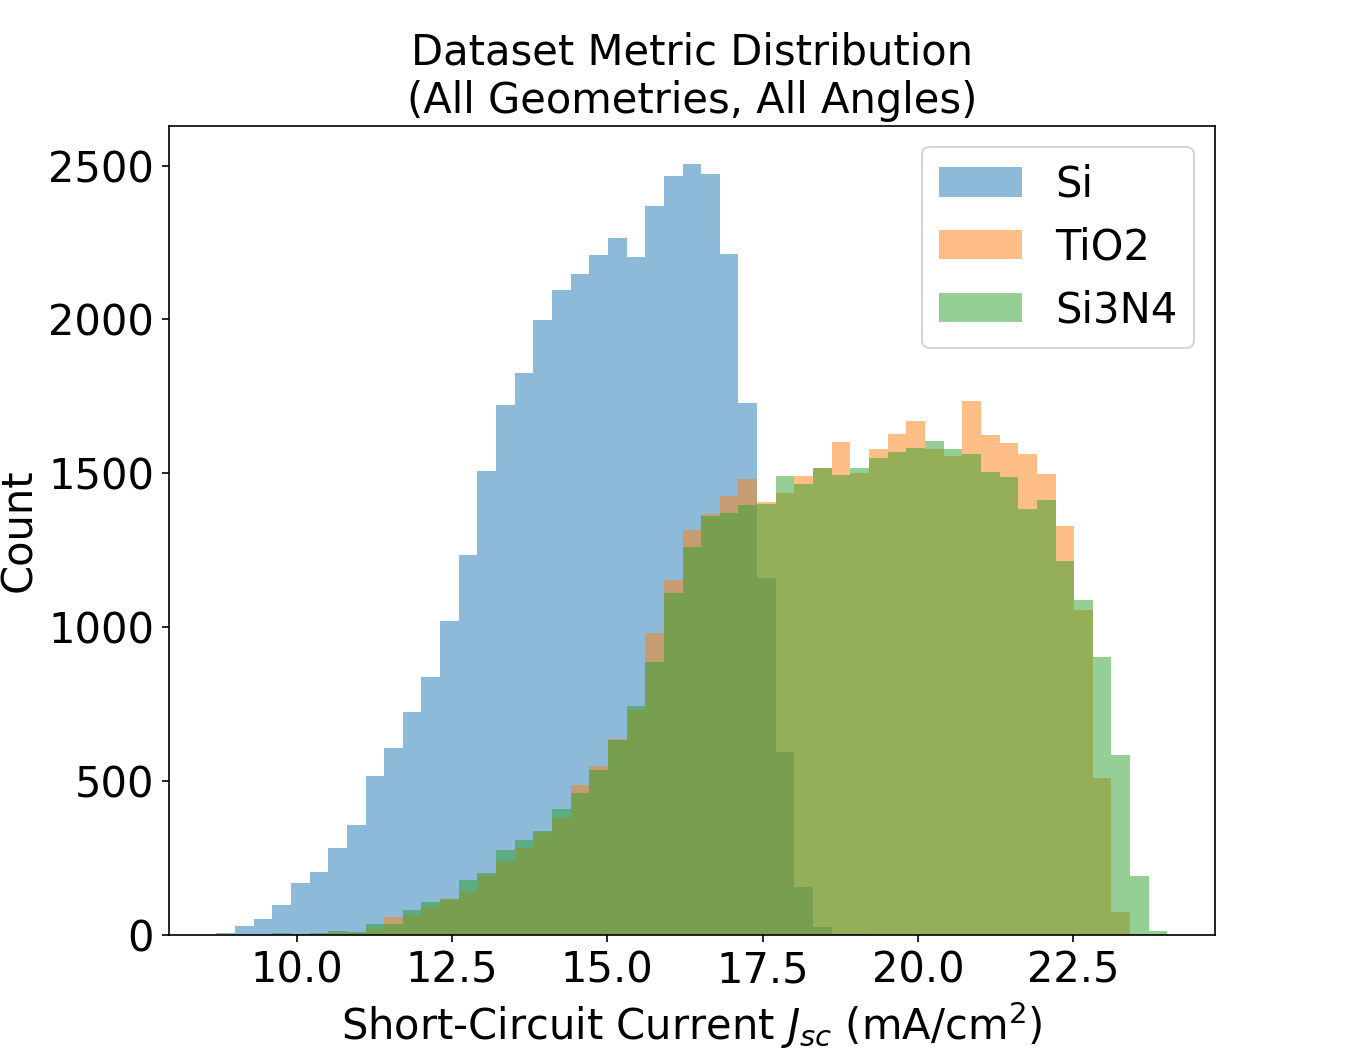
\includegraphics[width=\linewidth]{../Checkpoints/Si_TiO2_Si3N4/evaluation/dataset_baseline/jsc/dataset_metric_histogram.png}
        \caption{$J_{sc}$ histogram}
        \label{fig:jschist}
    \end{subfigure}
    \hfill % This command inserts flexible space between the figures
    % --- Second Subfigure ---
    \begin{subfigure}[b]{0.48\textwidth}
        \centering
        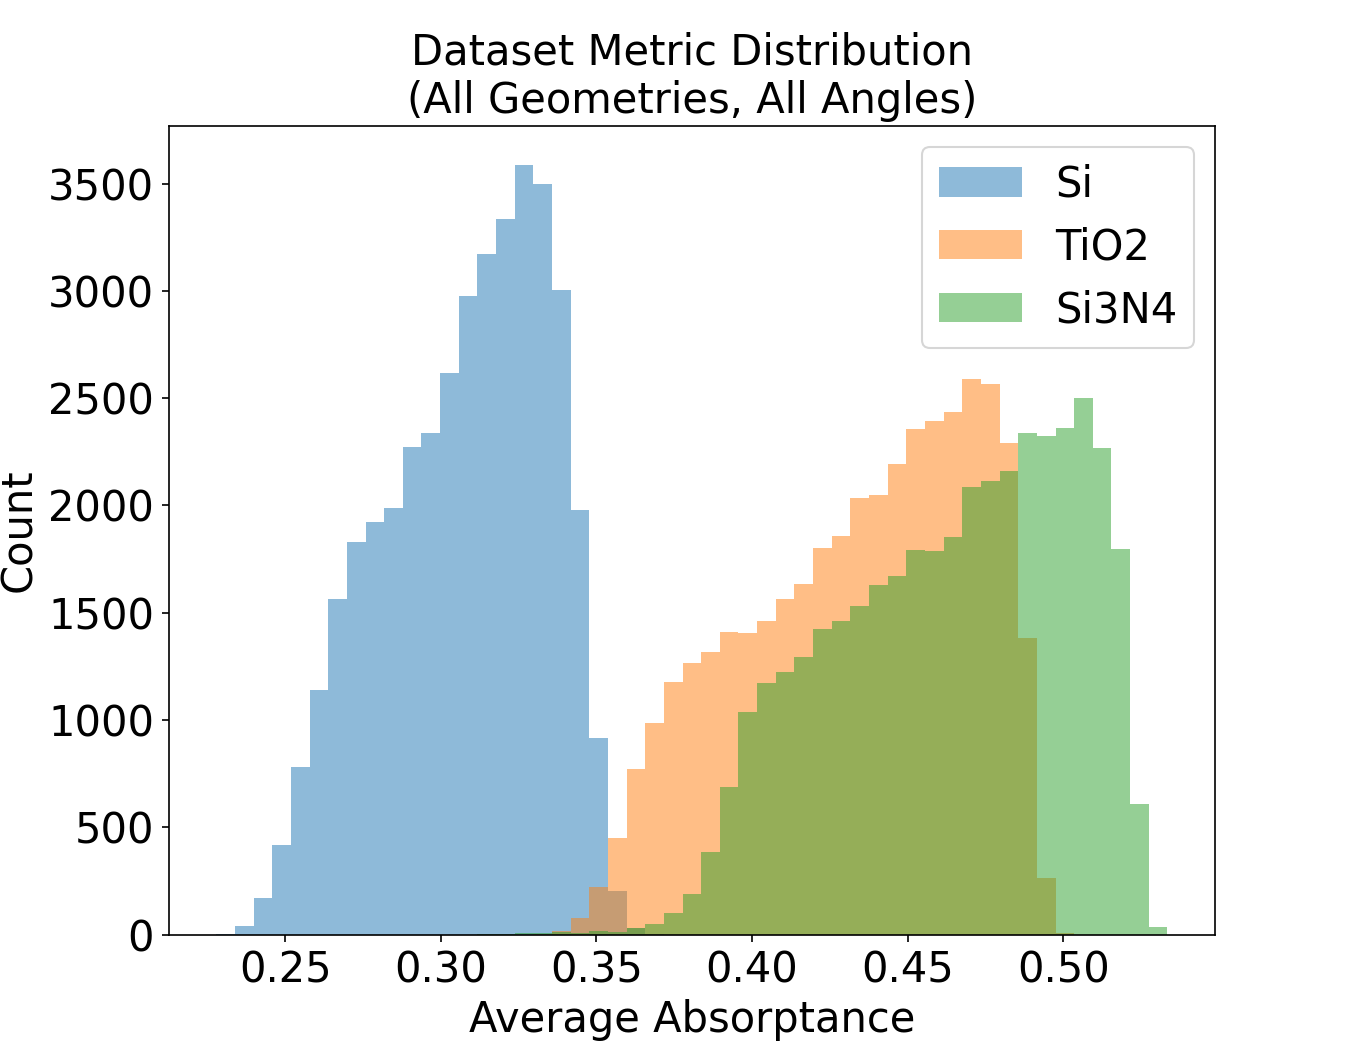
\includegraphics[width=\linewidth]{../Checkpoints/Si_TiO2_Si3N4/evaluation/dataset_baseline/all_data/dataset_metric_histogram.png}
        \caption{Average absorptance histogram}
        \label{fig:meanabshist}
    \end{subfigure}
    
    \caption{(a) A histogram over the full 2D dataset distritbution of Short-circuit currents.\newline (b) A histogram over the full 2D dataset distritbution of average absorptances}
    \label{fig:2dDatasetHists}
\end{figure}





\section{Surrogate Model Training}
Table \ref{tab:frac_models_stats} summarizes the training history of various surrogate models across different sizes of the dataset ($10\%$, $25\%$, $50\%$, and $100\%$). For each dataset configuration, three architectures were trained: an MLP baseline (\texttt{forward\_mlp}), a Convolutional Neural Network with skip connections (\texttt{skip\_cnn}), and a SIREN network.

\begin{table}[htbp]
    \centering
    \begin{tabular}{llccc}
    \toprule
    \textbf{Dataset Setup} & \textbf{Model Type} & \textbf{Test MAE} & \textbf{Test Max Err} & \textbf{Test R$^2$} \\
    \midrule
        Trained on 10\% train set & \texttt{forward\_mlp} & 0.1034 & 0.6288 & 0.7928 \\
         & \texttt{skip\_cnn} & \textbf{0.0510} & \textbf{0.4710} & \textbf{0.9094} \\
         & \texttt{siren} & 0.1007 & 0.8368 & 0.7484 \\
        \midrule
        Trained on 25\% train set & \texttt{forward\_mlp} & 0.0854 & 0.6987 & 0.7933 \\
         & \texttt{skip\_cnn} & \textbf{0.0300} & \textbf{0.3305} & \textbf{0.9732} \\
         & \texttt{siren} & 0.0331 & 0.3461 & 0.9673 \\
        \midrule
        Trained on 50\% train set & \texttt{forward\_mlp} & 0.0854 & 0.7117 & 0.7905 \\
         & \texttt{skip\_cnn} & 0.0297 & 0.3259 & 0.9738 \\
         & \texttt{siren} & \textbf{0.0285} & \textbf{0.3240} & \textbf{0.9755} \\
        \midrule
        Trained on 100\% train set & \texttt{forward\_mlp} & 0.0842 & 0.6840 & 0.7906 \\
         & \texttt{skip\_cnn} & \textbf{0.0253} & \textbf{0.3126} & \textbf{0.9794} \\
         & \texttt{siren} & 0.0283 & 0.3211 & 0.9750 \\
    \bottomrule
\end{tabular}

    \caption{Global statistics for surrogate models trained on fractional subsets of the Si-TiO$_2$-Si$_3$N$_4$ dataset. Mean Absolute Error (MAE), Maximum Absolute Error, and $R^2$ are evaluated on the full test dataset.}
    \label{tab:frac_models_stats}
\end{table}

\begin{figure}[htbp]
    \centering
    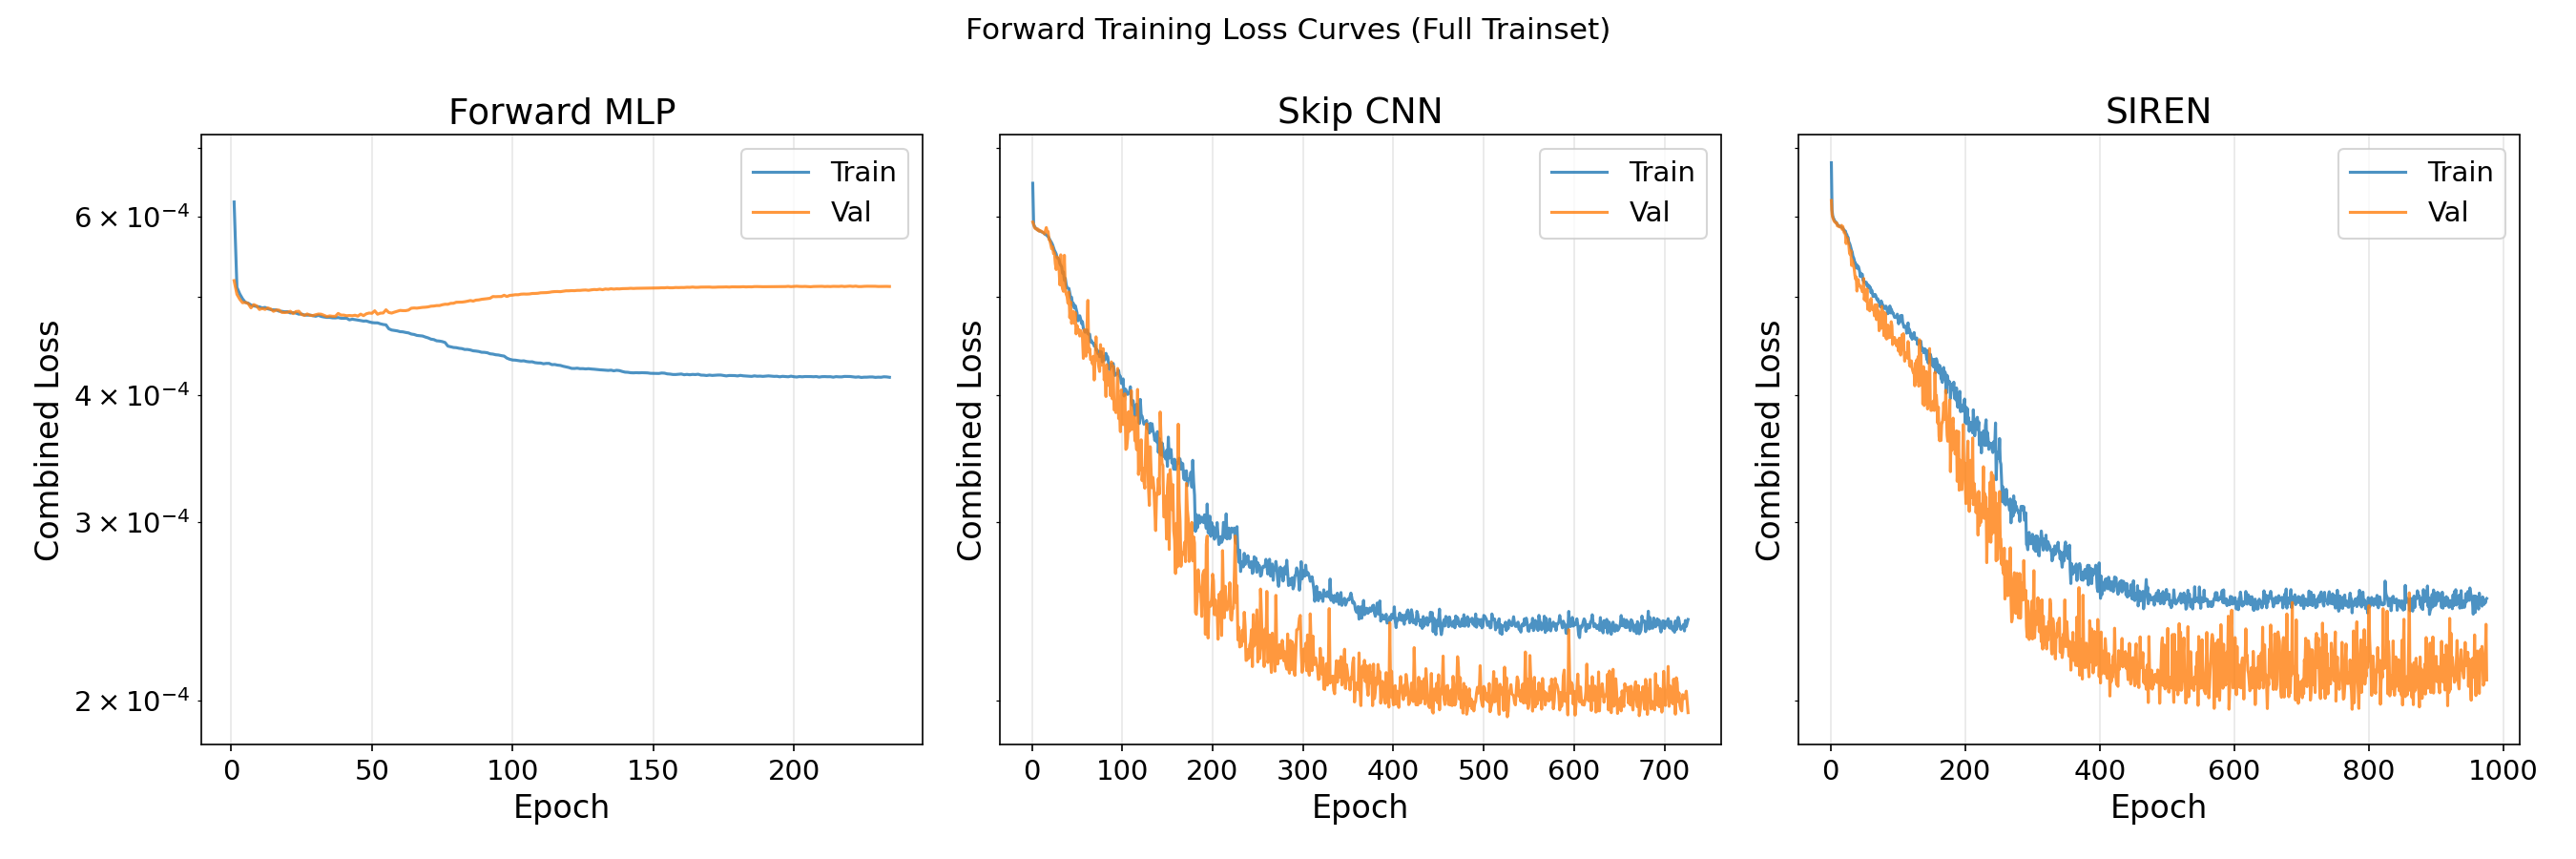
\includegraphics[width=0.9\textwidth]{figures/loss_curves/forward_loss_curves_Si_TiO2_Si3N4.png}
    \caption{Training and validation loss curves for the surrogate models trained on the full dataset (100\% train set).}
    \label{fig:loss_curves}
\end{figure}
\begin{table}[htbp]
    \centering
    \resizebox{\textwidth}{!}{%
    \begin{tabular}{lcccc}
        \toprule
        \textbf{Model} & \textbf{Sequential Total (s)} & \textbf{Batched Total (s)} & \textbf{Speedup (Sequential)} & \textbf{Speedup (Batched)} \\
        \midrule
        TORCWA & 1629.7 & -- & 1$\times$ & -- \\
        Skip CNN & 0.0351 & 0.0011 & 46,427$\times$ & 1,433,628$\times$ \\
        SIREN & 0.0213 & 0.0029 & 76,555$\times$ & 553,664$\times$ \\
        Forward MLP & 0.0041 & 0.0024 & 399,039$\times$ & 680,356$\times$ \\
        \bottomrule
    \end{tabular}%
    }
    \caption{Computational timing comparison between TORCWA and surrogate models for evaluating 10 sample structures. Surrogate models show massive acceleration, especially when batched.}
    \label{tab:timing_comparison}
\end{table}



\begin{table}[htbp]
    \centering
    \resizebox{\textwidth}{!}{%
    \begin{tabular}{lcccc}
        \toprule
        \textbf{Model} & \textbf{Sequential Total (s)} & \textbf{Batched Total (s)} & \textbf{Speedup (Sequential)} & \textbf{Speedup (Batched)} \\
        \midrule
        TORCWA & 1629.7 & -- & 1$\times$ & -- \\
        Skip CNN & 0.0351 & 0.0011 & 46,427$\times$ & 1,433,628$\times$ \\
        SIREN & 0.0213 & 0.0029 & 76,555$\times$ & 553,664$\times$ \\
        Forward MLP & 0.0041 & 0.0024 & 399,039$\times$ & 680,356$\times$ \\
        \bottomrule
    \end{tabular}%
    }
    \caption{Computational timing comparison between TORCWA and surrogate models for evaluating 10 sample structures. Surrogate models show massive acceleration, especially when batched.}
    \label{tab:timing_comparison}
\end{table}
